\subsection{Plastic plate - Rotational hardening plasticity (2D)}

\subsubsection*{Problem definition}

This example is a plane strain compression test on a
material with both isotropic and rotational hardening behaviour.

The geometry of the specimen used is $0.34$~m height and $0.1$~m
width. We denote by $\sigma_x$ the stress acting on the both
lateral sides of the specimen and by $\sigma_y$ the stress applied
to the top side of the specimen.
 The set-up of the problem is shown in Fig.~\ref{fig:ssy}.

\begin{figure}[H]
\center
\includegraphics[scale=0.3]{M/ssy_mesh.eps}
\caption{Plane strain biaxial test: rotational hardening}
 \label{fig:ssy}
\end{figure}

A vertical down displacement load is applied on the top boundary.

\subsubsection*{Material properties}

Assume all initial stresses are zero. The material properties of the rotational hardening model
are defined in Table \ref{Tab_par_oedo}
\begin{table}[!htb]
\centering
\begin{tabular}{lll}
\hline \hline
Parameter   &  Unit  & Value\\
\hline
  Young's modulus &  Pa &  1e+08 \\
\hline
  Poisson ratio & - &  0.3 \\
\hline
  $\alpha_0$       &  -        & 0.0 \\
  $\beta_0$        &  -        & 0.26 \\
  $\delta_0$       &  $m^2/N$  & 3.5e-07\\
  $ \varepsilon_0$ &  $m^2/N$  & 1.0e-7\\
  $\kappa_0$       &  $N/m^2$  & 0.0  \\
  $\gamma_0$       &  -        & 0.0 \\
  $m_0$            &  -        & 0.569 \\
\hline
  $\hat {\alpha}$  &  -        & 0.0 \\
  $\hat {\beta_0}$ &  -        & 0.29\\
  $\hat{\delta_0}$ &  $m^2/N$  & 8.81e-9\\
  $\hat{\varepsilon_0}$&  $m^2/N$  & 1.5e-8 \\
  $\hat{\kappa_0}$ &  $N/m^2$  & 0.0  \\
  $\hat{\gamma_0}$ &  -        & 0.0 \\
  $\hat{m_0}$      &  -        & 1.0 \\
\hline
  $\psi_1$         &   -       & 0.55\\
  $\psi_2$         &  -        & -0.26\\
\hline
  $C_h$            &  -        & 0.81e-3\\
  $C_d$            &  -        & 0.60e-3\\
\hline
  $b_r$            &  -        & 100.0\\
  $m_r$            &  -        & -3.0\\
\hline \hline
\end{tabular}
\caption{\label{Tab_par_oedo}Material parameters of rotational hardening
model }
\end{table}

\subsubsection*{Results}

The output of the results in a
specified point, i.e, a center of a finite element close to the
geometrical center of the domain (Fig.~\ref{fig:ssy}), is used to analyze the model behavior.
Fig. \ref{fig:ssy_u_s} shows the varying of vertical stress along with vertical displacement at the top boundary.

\begin{figure}[!htb]
\center
\includegraphics[scale=0.4]{M/ssy_u_s.eps}
\caption{Vertical stress vs vertical displacement}
 \label{fig:ssy_u_s}
\end{figure}

\subsubsection*{Benchmark deposit}

\begin{tabular}{|l|l|l|}
  \hline
  Benchmark & Problem type & Path in benchmark deposit \\
  \hline
 \emph{m\_ssy\_quad}& M & benchmarks\verb \M\ \\
  \hline
\end{tabular}
